% Proposed solution: processing element and MAC microarchitecture (issue #9; final-report update in #67).

\subsection{Processing Element and MAC Unit}
Each processing element (PE) owns one output element $C[i][j]$. It holds a multiply-accumulate unit (MAC) and two forwarding registers. The MAC multiplies two signed 8-bit operands into a 16-bit product, sign-extends that product to a 32-bit accumulator, and adds it to the running sum in every enabled cycle. The product is formed at its natural width before the sign extension, so the sign bit is never read as zero. Clear has priority over enable, and reset behaves like clear.

The PE also registers its operands. The left operand $a$ is copied to the right neighbour and the top operand $b$ to the neighbour below, one enabled cycle later. Each operand therefore moves one PE per cycle, which is what lets the skewed inputs meet at PE $(i,j)$ in the cycle that the term $A[i][k]B[k][j]$ needs. Fig.~\ref{fig:pe-wave} shows both behaviours in the PE testbench: the forwarded operands trail the inputs by one cycle, and four products accumulate to the expected dot product of 70.

\begin{figure*}[t]
\centering
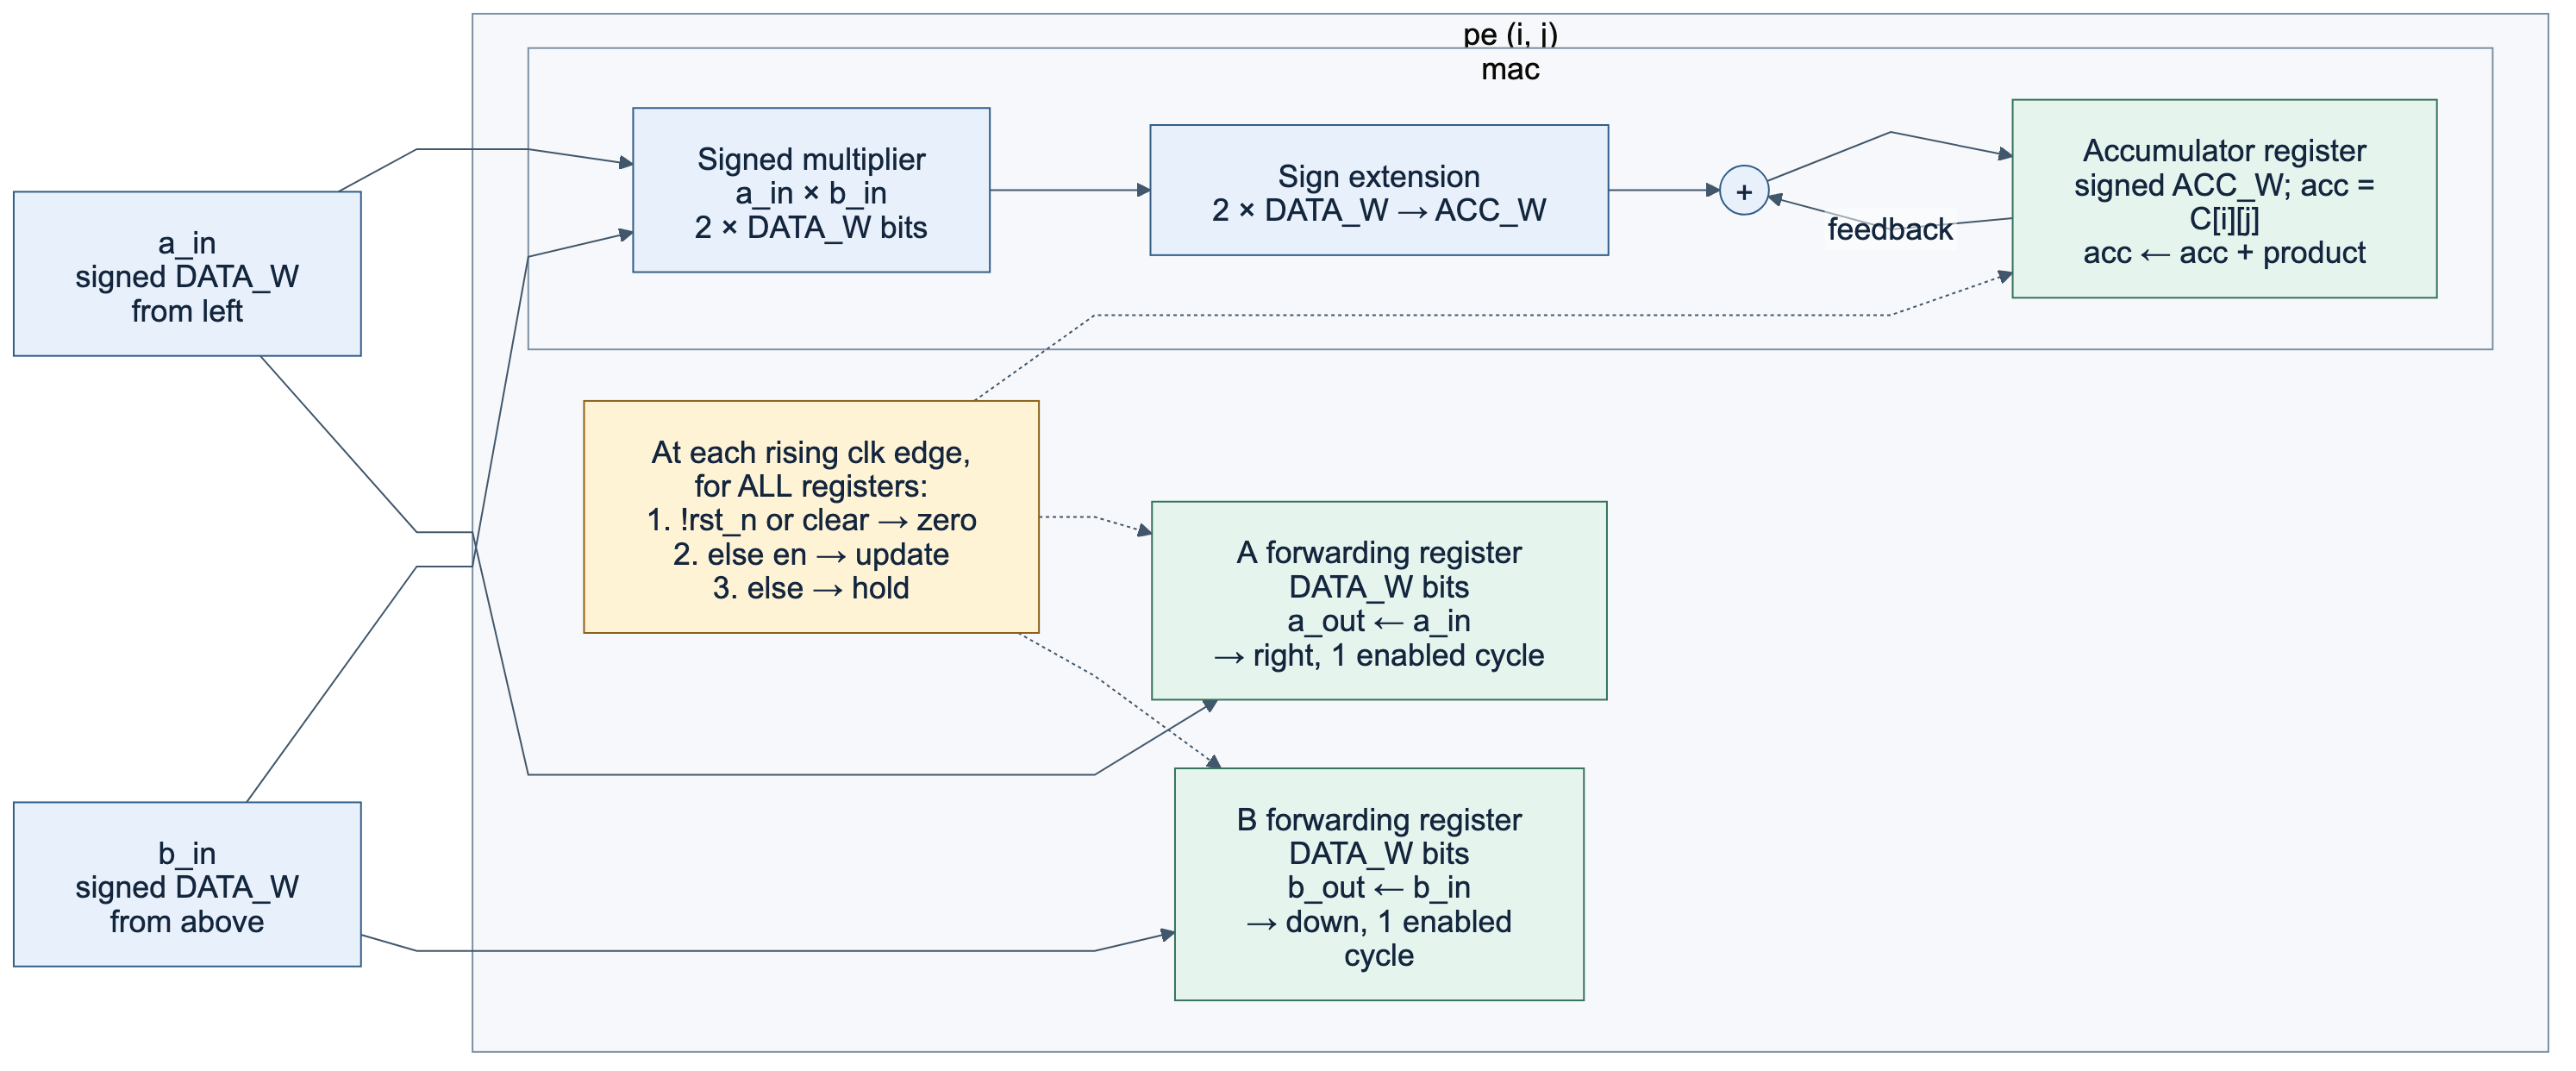
\includegraphics[width=\textwidth]{pe.png}
\caption{One PE in simulation (\texttt{tb\_pe}, GTKWave). Each operand leaves on \texttt{a\_out} and \texttt{b\_out} one enabled cycle after it arrives (A) and holds while \texttt{en} is low (B). The accumulator sums $1\cdot5 + 2\cdot6 + 3\cdot7 + 4\cdot8 = 70$ over $K = 4$ steps (C), and $-128 \times -128$ gives 16{,}384 (D).}
\label{fig:pe-wave}
\end{figure*}

The PE needed no change for Phase 2. A run with a shorter $k_{\mathrm{len}}$ simply enables it for fewer steps, and an accumulate run skips the clear, so the MAC keeps adding onto the sum of the previous run. A tiled product with inner dimension $K$ therefore builds each element of a tile in one accumulator, across all of its chunks.

The accumulator width follows from the largest possible sum. Over an inner dimension $K$, the largest magnitude is $K \cdot 2^{2\cdot\mathrm{DATA\_W}-2} = K \cdot 2^{14}$, reached when every operand is $-128$: 65{,}536 for $K = 4$, which needs 18 bits. A 32-bit accumulator holds this for any $K$ up to 131{,}071, however many chunks the product is split into, so the datapath does not saturate. Rounding and saturating the results back to 8 bits are out of scope.
